\begin{figure}[!htb]
    \centering
    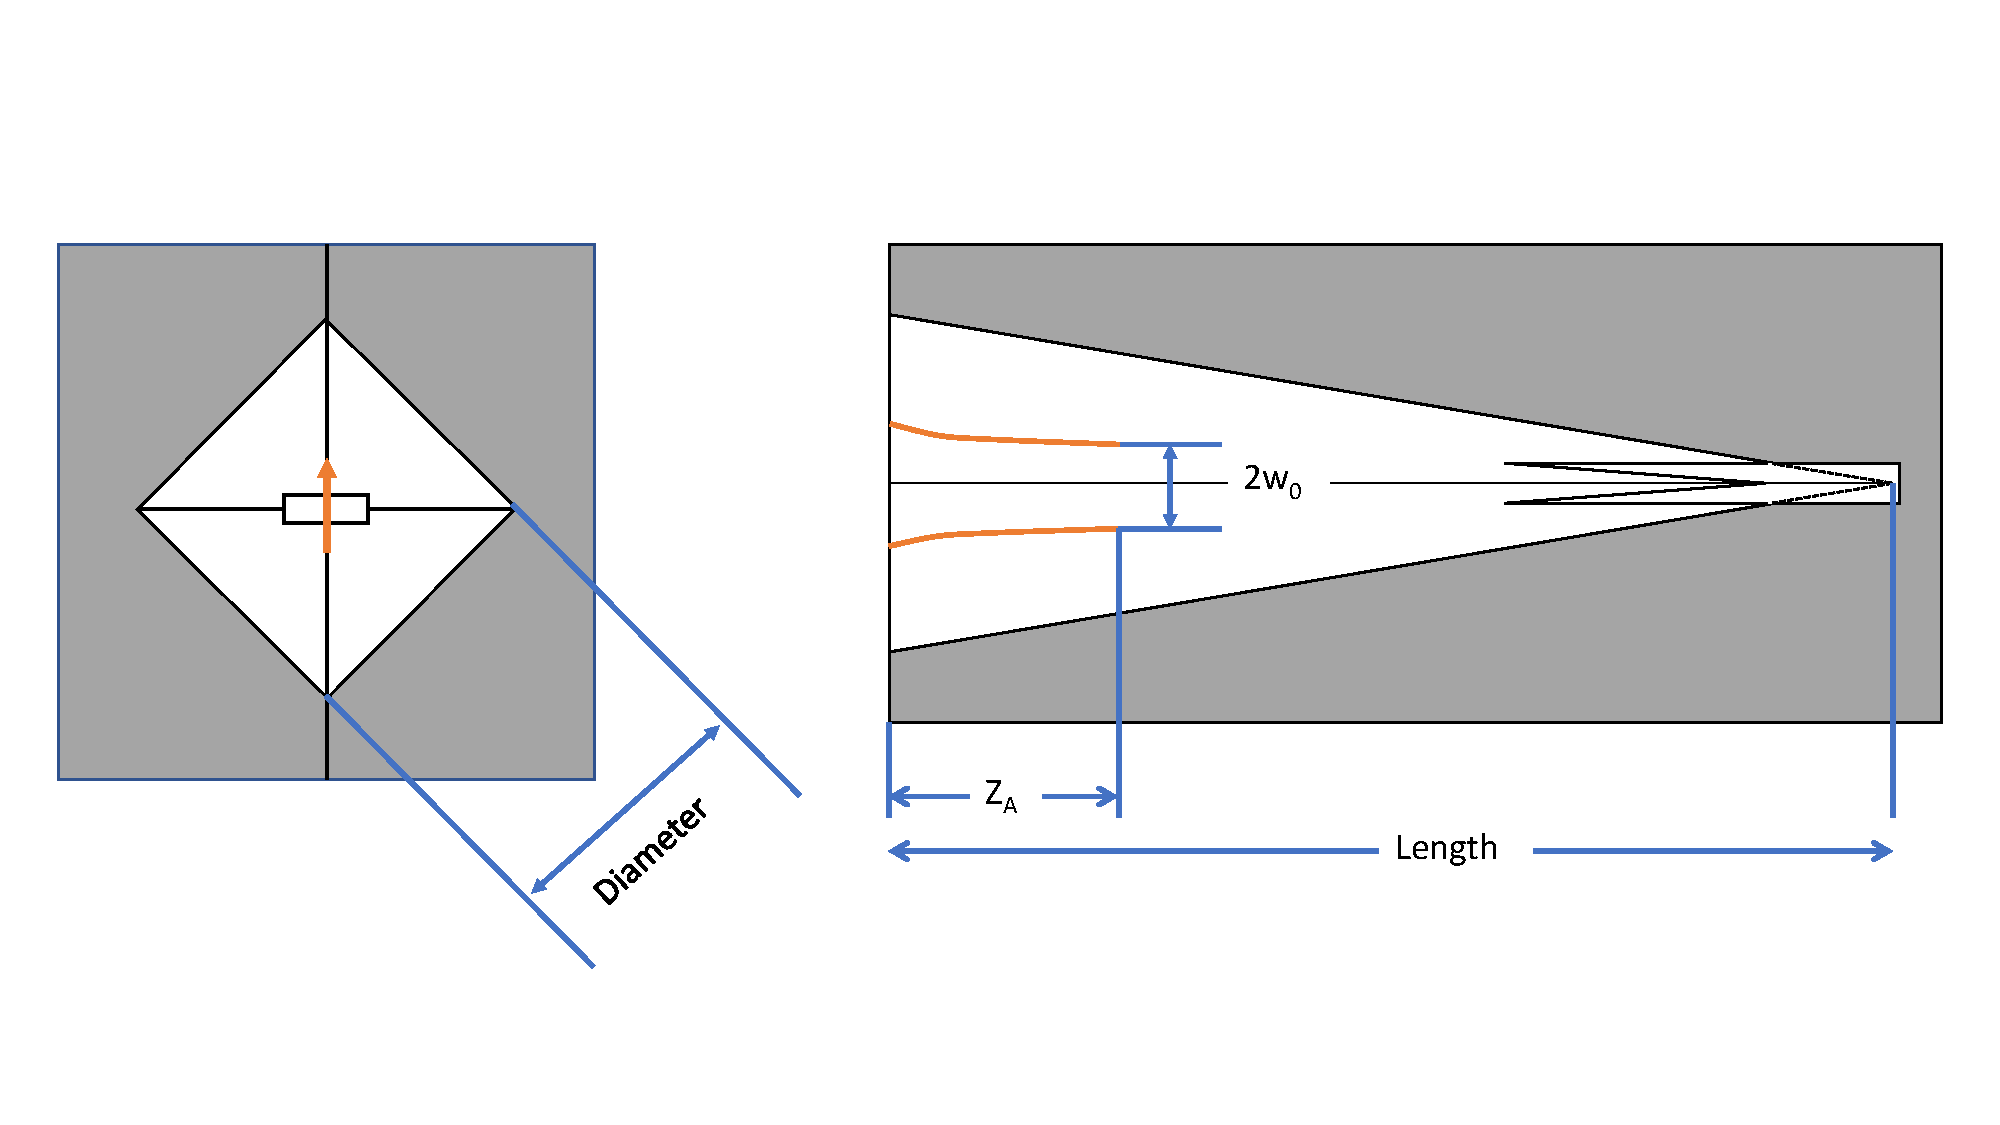
\includegraphics[width=0.9\textwidth]{figures/measurements/power-curve-453GHz/THz feed horn.pdf}
    \caption{Schematics of the nominal feed horn antenna are shown. Z$_A$ is defined as the location of the beam waist radius (w$_0$) with respect to the horn aperture. The upward arrow (orange solid line) indicates the polarisation direction of the electric field.}
    \label{fig:feed-horn}
\end{figure}